\chapter{Introdução}
%---------------------
% Edite a partir daqui 
%---------------------
Para editar a introdução, edite o arquivo introdução.tex na pasta textuais. Para chamar uma entrada do \gls{gls} use \verb+\gls{rótulo}+, chamando a entrada apropriada no arquivo postextuais/glossarios.tex.

Atente que esse modelo pode ser aplicado tanto ao TCC 1 quanto ao TCC 2, entretanto eles tem conteúdo diferente: 

\begin{minipage}{0.5\textwidth}
Conteúdo exigido do TCC 1
\end{minipage}
\begin{minipage}{0.5\textwidth}
Conteúdo exigido do TCC 2
\end{minipage}
\begin{minipage}{0.5\textwidth}

	\vspace{-15mm}
	\begin{itemize}
		\item introdução
		\item Justificativa
		\item Problematização
		\item Hipótese
		\item Objetivos
		\item Revisão bibliográfica
		\item Metodologia 
		\item Cronograma
		\item Referências
		\item Apêndices (opcional)
		\item Anexos (opcional)				
	\end{itemize}
\end{minipage}
\begin{minipage}{0.5\textwidth}
	\vspace{1cm}
	\begin{itemize}
		\item introdução
		\item Justificativa
		\item Problematização
		\item Hipótese
		\item Objetivos
		\item Revisão bibliográfica
		\item Metodologia 
		\item Proposta de trabalho
		\item Resultados
		\item Discussão
		\item Conclusão
		\item Referências
		\item Apêndices (opcional)
		\item Anexos (opcional)
	\end{itemize}
\end{minipage}

Capa, contracapa, folha de aprovação, listas de figuras, tabelas e o sumário são todos automaticamente gerados pelo \LaTeX   com base no que for incluído nos arquivos. O título do capítulo sempre será o que estiver incluso no comando \verb|\chapter{}| no início de cada capitulo. 

Notas de rodapé são incluídas com o comando:\par
\verb|\footnote{Texto da nota de rodapé}|\footnote{O texto da nota de rodapé é automaticamente numerado}.

A estrutura de arquivos que podem ou não ser incluídos está na sessão textual do arquivo \verb|TCC.tex|. Para omitir algum arquivo coloque um \verb|%| no inicio da linha onde ele é referenciado. 

\begin{figure}[!htb]
	\centering 
	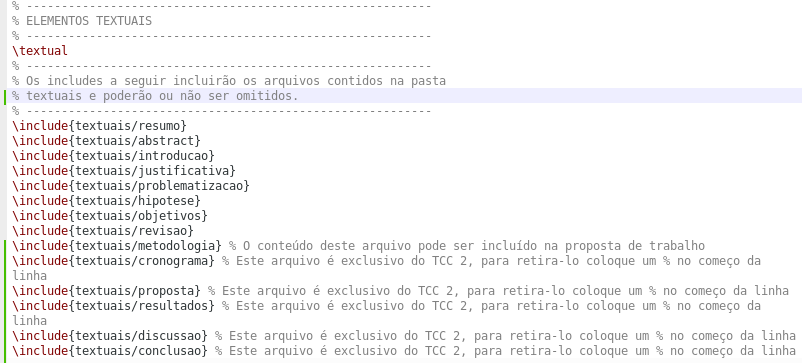
\includegraphics[width=\textwidth]{imagens/estrutura}
	\caption{Estrutura dos arquivos textuais}
	\label{fig:estrutura}
\end{figure}

Os dados da banca devem ser alterados no arquivo \verb|pretextuais/|\par\verb|folha_de_aprovacao.tex|.

\section{Ata e ficha catalográfica}

Após a aprovação do TCC pela banca alguns procedimentos devem ser tomados. 

\subsection{Ata}
Após a aprovação você receberá uma ata de aprovação. Para preparar o documento para catalogação e impressão você deve procurar no arquivo TCC.tex a linha a seguir: 
\par\verb|% ================================================================================
% Modelo da folha de aprovação, padrão UFPI, conforme modelo 
% disponível em https://drive.google.com/file/d/0B0BKqBVXhtedLWQzYVBhbUNRT1U/edit
% ================================================================================

\begin{folhadeaprovacao}
\begin{center}
	{\ABNTEXchapterfont\large\imprimirautor}
	\vspace*{\fill}\vspace*{\fill}
	\begin{center}
		\ABNTEXchapterfont\bfseries\Large\imprimirtitulo
	\end{center}
	\vspace*{\fill}
	\hspace{.45\textwidth}
	\begin{minipage}{.5\textwidth}
		\imprimirpreambulo
	\end{minipage}%
	\vspace*{\fill}
\end{center}

Trabalho \rule{4cm}{1pt}. \imprimirlocal, \rule{1cm}{1pt} de \rule{3cm}{1pt} de 2020:

% ===
% edite os nomes e cargos dos professores da banca
% ===
\assinatura{\textbf{\imprimirorientador} \\ Orientador}
\assinatura{\textbf{Nome do coorientador} \\ Coorientador}
\assinatura{\textbf{Professor} \\ Convidado 1}
\assinatura{\textbf{Professor} \\ Convidado 2}
\assinatura{\textbf{Professor} \\ Convidado 3}
\begin{center}
	\vspace*{0.5cm}
	{\large\imprimirlocal}
	\par
	{\large\imprimirdata}
	\vspace*{1cm}
\end{center}
\end{folhadeaprovacao}| \par

Você então deve incluir um \verb|%| no começo dela, comentando a linha inteira.

Você deve então copiar o arquivo da ata e colar na pasta pretextuais, alterar seu nome para ata.pdf e retirar o \verb|%| do começo da linha a seguir:  
\par\verb|% \includepdf[pages=-]{pretextuais/ata.pdf}| \par
Ao descomentar a linha você permite que a ata seja inclusa no documento final. 

\subsection{Ficha catalográfica}

Após a inclusão da ata o documento deve ser submetido a Biblioteca da UFPI para catalogação. O serviço atualmente é feito através do \href{http://sigaa.ufpi.br}{SIGAA}, menu \textbf{Biblioteca} $\rightarrow$ \textbf{Serviços ao usuário} $\rightarrow$ \textbf{Solicitar Ficha Catalográfica}, enviando a versão com a ata de aprovação. 

Ao receber a ficha catalográfica ela deve ser inserida após a folha de rosto. Para isso você deve procurar a linha a seguir: 
\par\verb|% 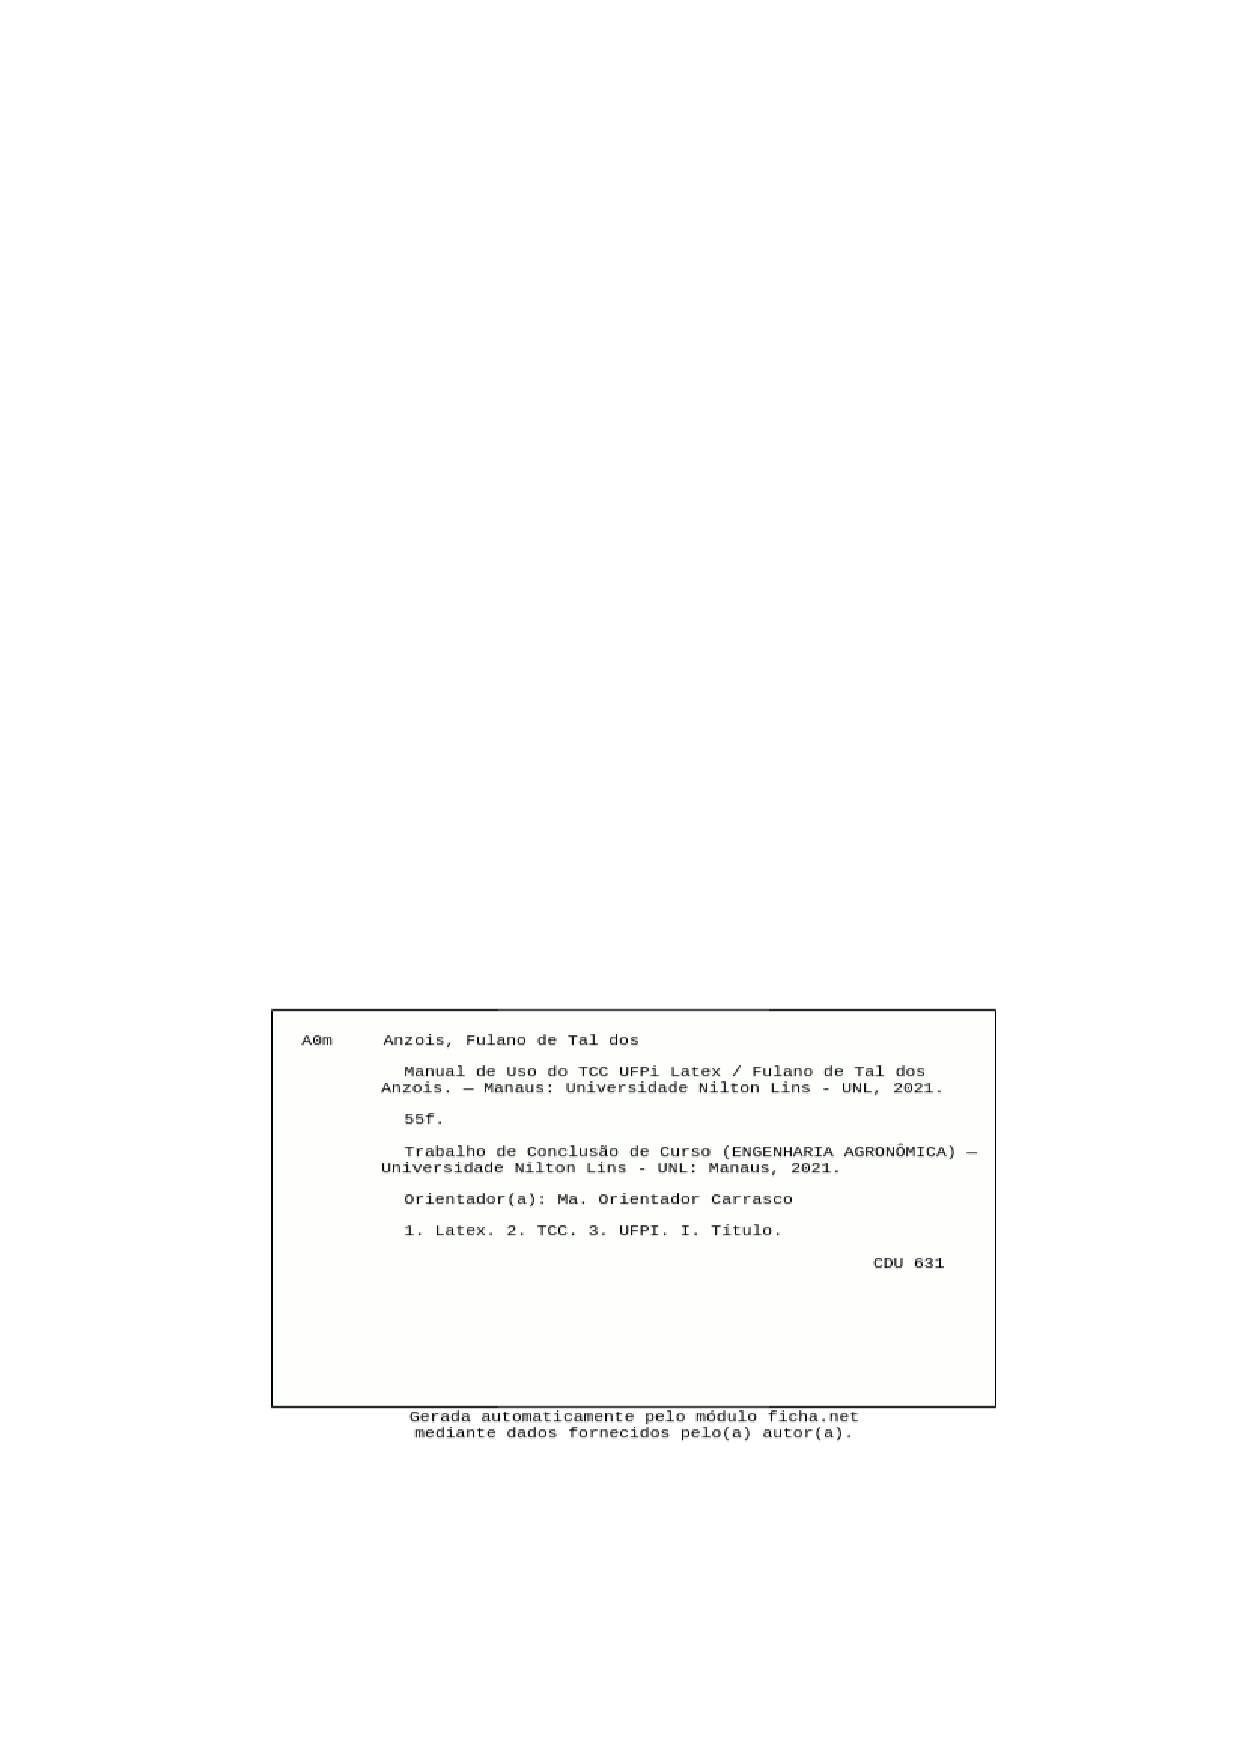
\includepdf[pages=-]{pretextuais/ficha_catalografica.pdf}| \par
Remova o \verb|%| do começo da linha. 

\section{Problemas conhecidos}

\subsection{Glossários com TeXstudio}
Há um problema conhecido com o \href{https://www.texstudio.org/}{TeXstudio}, que pula a geração de glossários em decorrência de um alerta do pdflatex, para corrigir o problema, execute os seguintes passos:

\begin{enumerate}
	\item Acesse a pasta \textbf{tcc-ufpi} usando o console.
	\item Execute o comando \verb|makeglossaries TCC|
	\item Verifique se houve a geração do arquivo \verb|TCC.gls| e \verb|TCC.glo|
	\item Volte ao TeXstudio e faça a compilação normalmente 
\end{enumerate}

Esse procedimento precisa ser repetido se houver alteração do arquivo glossarios.tex.


